%!TEX root = ../thesis.tex
\ifpdf
    \graphicspath{{Chapter2/Figs/Vector/}{Chapter2/Figs/PDF/}{Chapter2/Figs/}}
\else
    \graphicspath{{Chapter2/Figs/Raster/}{Chapter2/Figs/}}
\fi


\chapter{Theoretical Framework}
\label{chapter:theoretical-framework}

This chapter discusses Gaussian processes (GP) and deep Gaussian processes (DGPs), the composite model obtained by stacking multiple GP models on top of each other. We also review how to perform approximate Bayesian inference in these models, with a particular attention to Variational Inference. We also cover the theory of positive definite kernels and the Reproducing Kernel Hilbert Spaces (RKHS) they characterise.

\section{Gaussian Processes}
\label{sec:chapter1:gp}


Gaussian processes (GPs) \citep{rasmussen2006} are non-parametric distributions over functions similar to Bayesian Neural Networks (BNNs). The core difference is that neural networks represent distributions over functions through distributions on weights, while a Gaussian process specifies a distribution on function values at a collection of input locations. This representation allows us to use an infinite number of basis functions, while still enables Bayesian inference \citep{neal1996bayesian}. 

Following from the Kolmogorov extension theorem, we can construct a real-valued stochastic process (i.e. function) on a non-empty set $\mathcal{X}$, $f: \mathcal{X} \rightarrow \Reals$, if there exists on all finite subsets $\{x_1, \ldots x_N\} \subset \mathcal{X}$, a \emph{consistent} collection of finite-dimensional marginal distributions over $f(\{x_1, \ldots, x_n\})$. For a Gaussian process, in particular, the marginal distribution over every finite-dimensional subset is given by a multivariate normal distribution. This implies that, in order to fully specify a Gaussian process, it suffice to only define the mean and covariance (kernel) function because they are the sufficient statistics for every finite-dimensional marginal distribution. We can therefore denote the GP as
\begin{equation}
  \label{eq:chapter1:def-gp}
  f \sim \GP(\mu, k),
\end{equation}
where $\mu:\mathcal{X}\rightarrow\Reals$ is the mean function, which encodes the expected value of $f$ at every $x$, $\mu(x) = \Exp{f}{f(x)}$, and $k:\mathcal{X} \times \mathcal{X} \rightarrow \Reals$ is the covariance (kernel) function that describes the covariance between function values, $k(x, x') = \Cov\left(f(x), f(x')\right)$. The covariance function has to be a symmetric, positive-definite function. The Gaussianity, and the fact that we can manipulate function values at some finite points of interest without taking the behaviour at any other points into account (the marginalisation property) make GPs particularly convenient to manipulate and use as priors over functions in Bayesian models ---as we will show next.

Throughout this report, we will consider $f$ to be the complete function, and intuitively manipulate it as an infinitely long vector. When necessary, we will append `$(\cdot)$' to $f$ to highlight that it is indeed a function rather than a finite vector. Contrarily, $f(\vx) \in \Reals^N$ denotes the function evaluated at a finite set of points $\vx = \{x_1, \cdots, x_N\}$. $f^{\setminus \vx}$ denotes another infinitely long vector similar to $f$ but excluding $f(\vx)$. Intuitively, $f$ can be partitioned into two groups: $f(\vx)$ and $f^{\setminus \vx}$, with the following joint distribution
% Joint
\begin{equation}
  \begin{pmatrix} f^{\setminus \vx}(\cdot)\\ f(\vx) \end{pmatrix} \sim \NormDist{
    \begin{pmatrix} \mu(\cdot) \\ \vmu_{\vf} \end{pmatrix},
    \begin{pmatrix} k(\cdot, \cdot)  & \kfx\transpose \\ \kfx & \Kff \end{pmatrix},
  }
\end{equation}
where $[\vmu_\vf]_{i} = \mu(x_i)$, $[\Kff]_{i,j} = k(x_i, x_j)$, $[\kfx]_i = k(x_i, \cdot)$, and $\mu(\cdot)$ and $k(\cdot, \cdot)$ are the mean and covariance function from \cref{eq:chapter1:def-gp}. Following the marginalisation property, the distribution over $f(\vx)$ is given by
\begin{equation}
p(f(\vx)) = \int p(f)\,\calcd{f^{\setminus \vx}} = \NormDist{\vmu_{\vf}, \Kff}.
\end{equation}
% Condition
We can now specify the GP at this finite set of points and use the rules of conditioning to obtain the GP elsewhere. Let $f(\vx) \shorteq \vf$, then the conditional distribution for $f^{\setminus \vx}$ is given by another Gaussian process
\begin{equation}
  \label{eq:chapter1:conditional}
  p(f^{\setminus \vx}(\cdot) \given f(\vx) \shorteq \vf) = \GP\Big(\mu(\cdot) + \kfx^\top \Kff^{-1} (\vf - \vmu_{\vf}),\ \ k(\cdot, \cdot) -  \kfx^\top \Kff^{-1} \kfx\Big),
\end{equation}
The conditional distribution over the whole function $p(f(\cdot) \given f(\vx) = \vf)$ has the exact same form as in \cref{eq:chapter1:conditional}. This is mathematically slightly confusing because the random variable $f(\vx)$ is included both on the left and right-hand-side of the conditioning, but the equation is technically correct, as discussed in \citet{matthews16,van2020framework,Leibfried2020Tutorial}.

\subsection{The Beauty of Gaussian Process Regression: Exact Bayesian Inference}
\label{sec:gp-exact-inference}

A defining advantages of GPs is that we can perform exact Bayesian inference in the case of regression. % In this section we briefly discuss the general methodology of Bayesian modelling and how this is performed by GPs.
% \paragraph{Problem Defintion} 
Assume a supervised learning setting where $x \in \mathcal{X}$ (typically, $\mathcal{X} = \Reals^d$) and $y \in \Reals$, and we are given a dataset $\data = \{(x_i, y_i)\}_{i=1}^N$ of input and corresponding output pairs. For convenience, we sometimes group the inputs in $\vx = \{x_i\}_{i=1}^N$ into a single design matrix and outputs $\vy = \{y_i\}_{i=1}^N$ into a vector. We further assume that the data is generated by an unknown function $f: \mathcal{X} \rightarrow \Reals$, and that the outputs are perturbed versions of functions evaluations at the corresponding inputs: $y_i = f(x_i) + \epsilon_i$. In the case of regression we assume a Gaussian noise model $\epsilon_i \sim \NormDist{0, \sigma^2}$. We are interested in learning the function $f$ that generated the data. % We denote the evaluation of the function at all inputs as $f(\vx) \in \Reals^N$ and at a single input as $f(x_i) \in \Reals$.

% The key idea in Bayesian modelling is to specify a prior distribution over the quantity of interest. The prior encodes what we know at that point in time about the quantity. In general term, this can be a lot or a little. We encode this information in the form of a distribution. Then, as more data becomes available, we use the rules of probability, an in particlar Bayes' rule, to update our prior beliefs and compute a posterior distribution (see \citet{mackay2003information, bisschop} for a thorough introduction).

Following the Bayesian approach, we specify a \emph{prior} over the parameters of interests, which in the case of GPs is the function itself. The prior is important because it characterises the search space over possible solutions for $f$. Through the prior, we can encode strong assumptions, such as linearity, differentiability, periodicity, etc. or any combination thereof. These strong inductive biases make it possible to generalise well from very limited data. Compared to Bayesian parametric models, it is much more convenient and intuitive to specify priors directly in \emph{function-space}, rather than on the weights of a parametric model \citep{rasmussen2006}. 

In Gaussian process regression (GPR), we specify a GP prior over $f$, for which we assume without loss of generality a zero mean function:
\begin{equation}
  f \sim \GP\big(0, k\big),
\end{equation}
The likelihood, describing the relation between the quantity of interest $f$ and the observed data, is given by 
\begin{equation}
  \label{eq:likelihood}
  p(\vy \given f) = \prod_{i=1}^N p(y_i \given f) = \prod_{i=1}^N \NormDist{y_i \given f(x_i), \sigma^2},
\end{equation}
where we see that, conditioned on the GP, the likelihood factorises over datapoints. The posterior over the complete function $f$ is another GP, which can be obtained using Bayes' rule:
\begin{equation}
  \label{eq:f-given-y}
  p(f \given \vy) 
      = \GP\Big(\kfx^\top (\Kff + \sigma^2 \Eye)^{-1} \vy,\ \ k(\cdot, \cdot) -  \kfx^\top (\Kff + \sigma^2 \Eye)^{-1} \kfx\Big).
\end{equation}
Similarly, the marginal likelihood (model evidence) is also available in closed-form and obtained by marginalising over the prior:
\begin{equation}
  \label{eq:log-marginal-likelihood}
  p(\vy) = \NormDist{\vy \given \vzero, \Kff + \sigma^2 \Eye}.
\end{equation}
The availablility of the posterior and the marginal likelihood in analytic form makes GPs a unique tool for inferring unknown functions from data. 
% TODO: The marginal Occam's razor [Rasmussen and Ghahramani, 2001]

Despite the convenience of the analytic expressions, computing this exact posterior requires inverting the $N \times N$ matrix $\Kff$, which has a $\BigO(N^3)$ computational complexity and a $\BigO(N^2)$ memory footprint. Interestingly, the computational intractability in GPR models originates from the prior and \emph{not} the complexity of marginalisation as is often the case for other Bayesian methods [TODO: CITE]. Indeed, these methods resort to MCMC to avoid computing intractable normalising constant, which is a problem that GPR does not encounter.  Another shortcoming of GPR models is that there is no known analytical expression for the posterior distribution when the likelihood (\cref{eq:likelihood}) is not Gaussian, as encountered in classification for instance. In the next paragraph we discuss solutions to both problems.

\section{Approximate Inference with Sparse Gaussian Processes}

Sparse Gaussian processes combined with Variational Inference (VI) provide an elegant way to address these two shortcomings \citep{titsias2009, hensman2013, hensman2015scalable}. VI consists of introducing a distribution $q(f)$ that depends on some parameters, and finding the values of these parameters such that $q(f)$ gives the best possible approximation of the exact posterior $p(f \given \vy )$. It is worth noting that there exists other approaches in the literature that address the same issues. In particular, Expectation Propagation (EP) \citep{minka2001expectation,bui2017unifying} formulates, similar to VI, an approximation to the posterior but uses a different objective to optimise the approximation. Tangentially, other sparse GP methods (e.g., FITC) \citep{Snelson05,quinonero2005unifying} approximate the model rather than the posterior. A downside of this is that the posteriors lose their non-parametric nature, which can be detrimental for the uncertainty estimates \citep{bauer2016understanding}. In what follows we will focus on Sparse Gaussian processes with variational inference because of its general applicability and overall robust performance.

We first discuss the objective used in general variational inference before specifying our particular choice for $q(f)$. Let us therefore define $q(f)$ as the approximate to the posterior, then the idea is to optimise $q(f)$ so that the distance measured by the Kullback–Leibler (KL) divergence from $q(f)$ to $p(f \given \vy)$ is minimal. Rewriting $p(f \given \vy)$ using Bayes' rule, we obtain:
\begin{equation}
  \KL{q(f)}{p(f \given \vy)} = -{\Exp{q(f)}{\log \frac{p(\vy \given f) p(f)}{q(f)}}} + \log p(\vy).
\end{equation}
Rearranging these terms yields:
\begin{equation}
  \label{eq:elbo}
  \log p(\vy) - \KL{q(f)}{p(f \given \vy)} = 
  \underbrace{\Exp{q(f)}{\log p(\vy \given f)} - \KL{q(f)}{p(f)}}_{\triangleq\,\textrm{ELBO}}
\end{equation}
The r.h.s. of \cref{eq:elbo} is known as the Evidence Lower BOund (ELBO). It is a lower bound to the log marginal likelihood ($\log p(\vy)$) because the KL between $q(f)$ and $p(\vy \given f)$ is always non-negative. Further, since $p(\vy)$ does not depend on the variational approximation, maximising the ELBO w.r.t. $q(f)$ is equivalent to minimsing the $\KL{q(f)}{p(f \given \vy)}$. The maximum will be reached when $q(f) \shorteq p(f \given \vy)$, in which case the KL will be zero and the ELBO equals the log evidence. 

Intuitively, VI casts the problem of Bayesian inference, namely marginalisation, as an optimisation problem. The objective for the optimisation problem is the ELBO, which depends on the variational approximation, the prior and the data but, importantly, not the true posterior. This approach has several advantages. Firstly, optimisation, as opposed to marginalisation, is garantueed to converge ---albeit possibly to a local optima. Secondly, VI provides a framework in which one can trade computational cost for accuracy: by expanding the family of approximating distributions we can only tighten the bound. An interesting example of this is importance weighting, where in the limit of infinite compute the true posterior is part of the approximating family \citep{Domke2018IWVI}. Finally, the bound and its derivates can be computed with stochastic estimations using the reparametrisation trick or score function estimators which enables big data settings.

So far we have discussed the bound in VI, but have left $q(f)$ unspecified, we now focus our attention to this. In general, we want the family of variational distributions to be flexible enough, such that some setting of the parameters can approximate the true posterior well, while also being computationally efficient and mathematically convenient to manipulate. % Mark van der Wilk discusses in his thesis \citep{vdw2019thesis} also the importance of  maintaining the non-parametric uncertainty in the approximation. 
We follow the approach proposed by \citet{titsias2009}, which parameterises the approximation using a set of $M$ pseudo inputs $\vz = \{z_1, \ldots, z_M\} \in \Reals^{M \times d}$ corresponding to $M$ inducing variables $\vu = f(\vz) \in \Reals^M$. 
We choose to factorise the variational approximation as $q(f, \vu) = q(\vu) p(f\given f(\vz) \shorteq \vu)$, where
\begin{equation}
  p(f \given f(\vz) \shorteq \vu) = \GP\Big(\kux^\top \Kuu^{-1}\vu,\ \ k(\cdot, \cdot) -  \kux^\top \Kuu^{-1} \kux\Big), 
\end{equation}
with $[\Kuu]_{i,j} = k(z_i, z_j)$, $[\kux]_i = k(z_i, \cdot)$. We specify a Gaussian distribution for the variational posterior over the inducing variables with a freely parameterised mean and covariance
\begin{equation}
  q(\vu) = \NormDist{\vm, \MS}
\end{equation}
such that the overall approximate posterior is given by another GP
\begin{equation}
  \label{eq:qf}
  q(f) = \int_{\vu} q(f, \vu)\,\calcd{\vu} = \GP\Big(\kux^\top \Kuu^{-1}\vm,\ \ k(\cdot, \cdot) -  \kux^\top \Kuu^{-1} (\Kuu + \MS)\Kuu^{-1} \kux\Big).
\end{equation}
as a result of the conjugacy of the variational posterior $q(\vu)$ and the conditional. 
The approximation admits several interesting properties. Firstly, in the case of a Gaussian likelihood and the number of inducing points that equals the amount of data, $q(f)$ contains the true posterior. That is, if $\vz \shorteq \vx$, it is possible to set $\vm$ and $\MS$ such that $q(f) = p(f \given \vy)$ \citep{titsias2009}. Secondly, \citet{burt2019} showed that for $N \rightarrow \infty$, the approximate posterior can be made arbitrarly close to the true posterior for $M = \BigO(\log N)$. Finally, we notice that the approximate mean exhibits the same structure as a parametric model with basis functions $\kux$ and weights $\Kuu\inv \vm$. The variance, however, remains non-parametric, which means that predictions are made with an infinite amount of basis functions---exactly like in the true posterior. For non-degenarate kernels, this leads to error bars that are unconstrained by the data. We will come back to the parameteric nature of the approximate mean in \cref{chapter:dnn-as-point-estimate-for-dgps}.

We optimise the variational parameters $\{\vm, \MS\}$ by maximising the ELBO \cref{eq:elbo}. Assuming a general likelihood of the form $p(\vy \given f) = \prod_i p(y_i \given f(x_i))$ the objective can be written as
\begin{equation}
  \label{eq:elbo-gp} 
  \textrm{ELBO} = \sum_{i=1}^N \Exp{q(f(x_i))}{\log p(y_i \given f(x_i))} - \KL{q(\vu)}{p(\vu)} \,. 
\end{equation}
Crucially, the original KL between the two infinite-dimensional processes $\KL{q(f)}{p(f)}$ is mathematically equivalent to the finite-dimensional KL between the variational posterior and prior over the inducing variables. We refer the interested reader to \citet{matthews16} for a theoretical analysis of the equivalence and to \citet[Section 4.1]{Leibfried2020Tutorial} for a more intuitive explanation. The objective in \cref{eq:elbo-gp}, introduced in \citet{hensman2013,hensman2015scalable} reduces the computational complexity to $\BigO(M^2 N + M^3)$. It also allows for stochastic estimation through minibatching \citep{hensman2013} and for non-Gaussian likelihoods through Gauss-Hermite quadrature of the one-dimensinoal expectation over $q(f(x_i))$ \citep{hensman2015scalable}.

\subsection{Interdomain Inducing Variables}
\label{section:interdomain-inducing-variables}

Interdomain Gaussian processes use alternative forms of inducing variables such that the resulting sparse GP models consists of a different set of features. %\cref{chapter:vish} and \cref{chapter:dnn-as-point-estimate-for-dgps} heavily rely on this paradigm. 
Classically, inducing variables are defined as pseudo function evaluations: $u_m = f(z_m)$, but in interdomain GPs the inducing variables are obtained using a linear transformation of the GP: $u_m = \mathcal{L}_m f$. This redefinition of $\vu$ implies that the expressions of $\Kuu$ and $\kux$ change, but the inference scheme of interdomain GPs and the mathematical expressions for the posterior mean and variance are exactly the same as classic sparse GPs. This is thanks to the linearity of the operator and the preservation of (joint) Gaussian behaviour under linear transformations. A common linear operator is the integral operator with an inducing function $g_m$ \citep{lazaro2009inter}:
\begin{equation*}
    \mathcal{L}_m\,f = \int f(x)\,g_m(x)\,\calcd{x}\,.
\end{equation*}
In this case, $\Kuu$ and $\kux$ take the form
\begin{equation}
 [\Kuu]_{m,m'}  = \Cov(\mathcal{L}_m f, \mathcal{L}_{m'} f) = \int\!\int k(x, x') g_{m}(x) g_{m'}(x') \calcd{x}\,\calcd{x'}
\end{equation}
and 
\begin{equation}
 [\kux]_{m}  = \Cov(\mathcal{L}_m f, f)) = \int k(\cdot, x') g_{m'}(x') \calcd{x'}.
\end{equation}

Most current interdomain methods are designed to improve computational properties \citep{hensman2017variational,Dutordoir2020spherical,burt2020variational}. For example, Variational Fourier Features (VFF)~\citep{hensman2017variational} is an interdomain method where the inducing variables are given by a Mat\'ern RKHS inner product between the GP and elements of the Fourier basis:
\begin{equation*}
u_m = \langle f, \psi_m \rangle_\rkhs,
\end{equation*}
where $\psi_0 = 1$, $\psi_{2m}=\cos(m x)$ and $\psi_{2m+1}=\sin(m x)$ if the input space is $[0, 2 \pi]$. This leads to
\begin{equation*}
    \Kuu = \left[\langle \psi_i , \psi_{j} \rangle_\rkhs^{} \right]_{i, j = 0}^{M-1}\qquad\text{and}\qquad\kux = \left[ \psi_i(x)\right]_{i = 0}^{M-1}\, .
\end{equation*}
This results in several advantages. First, the features $\kux$ are exactly the elements of the Fourier basis, which are independent of the kernel parameters and can be precomputed. Second, the matrix $\Kuu$ is the sum of a diagonal matrix plus low rank matrices. This structure can be used to drastically reduce the computational complexity, and the experiments showed one or two orders of magnitude speed-ups compared to classic sparse GPs. Another reason to use interdomain inducing variables is the ability is gives to control $\kux$---as shown in the next example.

\subsubsection*{Example: Heavyside Inducing Variable}


\begin{figure}[tbh!]
  \centering
\begin{subfigure}{0.3\textwidth}
  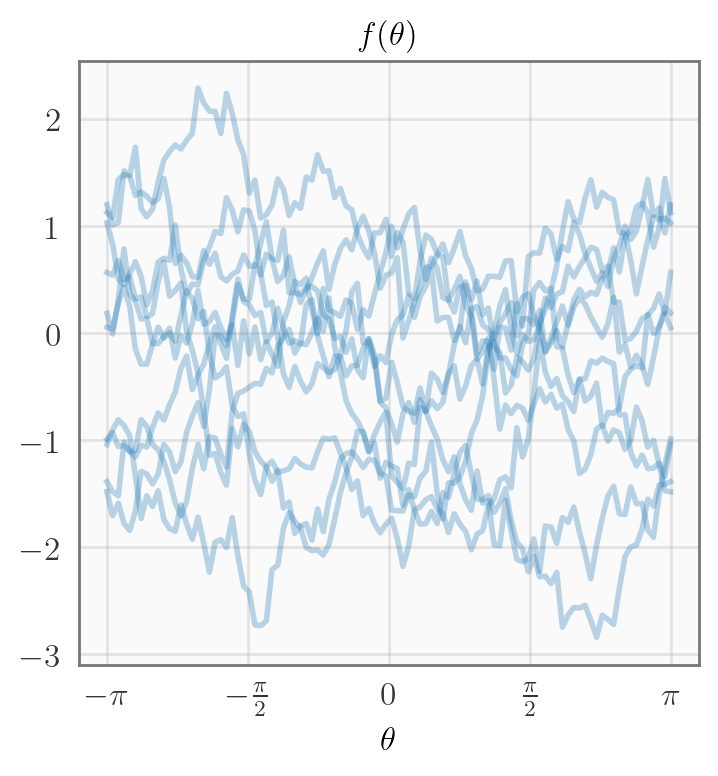
\includegraphics[width=\textwidth]{heaviside2}
  \caption{Samples}
  \label{fig:heaviside1}
\end{subfigure}\hfil % <-- added
\begin{subfigure}{0.3\textwidth}
  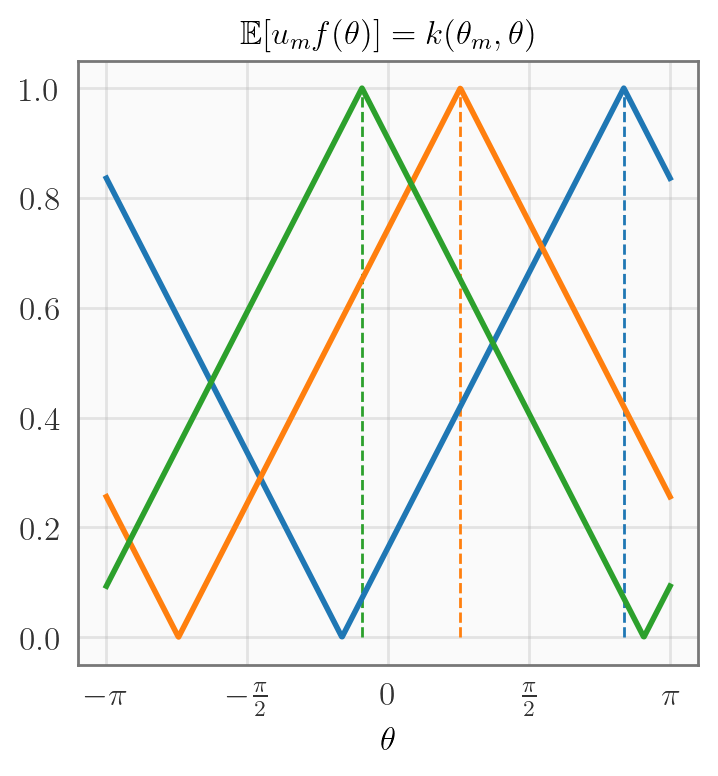
\includegraphics[width=\textwidth]{heaviside1}
  \caption{$u_m = f(\theta_m)$}
  \label{fig:heaviside2}
\end{subfigure}\hfil % <-- added
\begin{subfigure}{0.3\textwidth}
  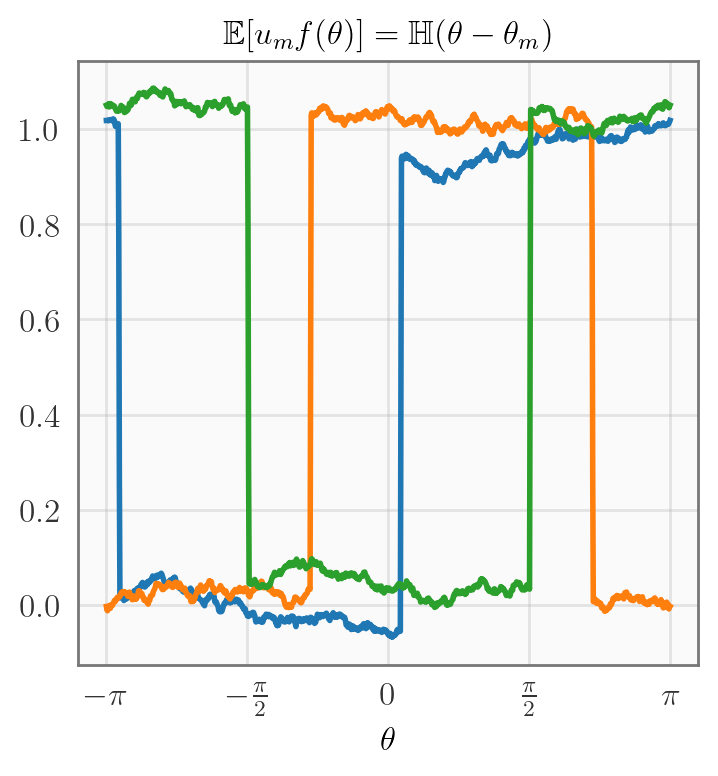
\includegraphics[width=\textwidth]{heaviside3}
  \caption{$u_m = \mathcal{L}_m f$}
  \label{fig:heaviside3}
\end{subfigure}
\caption{Example of interdomain inducing variables for the first-order Arc Cosine kernel.}
\label{fig:images}
\end{figure}

Using interdomain inducing variables in Sparse Variational Gaussian processes makes it possible to construct approximate GPs in which the basis functions exhibit interesting behaviour. As an illustration, in this example we design an inducing variable, through a linear transformation of the GP, for which the basis functions $\kux$ are given by the Heavide function. Therefore, assume $f \sim \GP(0, k)$ defined on $\sphere^1$ (the unit circle), $f: [-\pi, \pi] \rightarrow \Reals, \theta \mapsto f(\theta)$ and $k$ the zero-th order Arc Cosine kernel \citep{cho2009kernel}, defined as:
\begin{equation}
  k(\theta, \theta') = 1 - \frac{\varphi}{\pi},
\end{equation}
where $\varphi \in [0, \pi]$ is the shortest angle between the two inputs. In \cref{fig:heaviside1} we show samples from this GP and in \cref{fig:heaviside2} we plot $k(\theta_m, \theta)$ for three different values of $\theta_m$.

Let us now define the $m$-th linear operator as the sum of the derivate at $\theta_m$ and the integral over the domain:
\begin{equation}
  \mathcal{L}_m = \frac{\calcd{}}{\calcd{\theta}}\Bigr|_{\theta = \theta_m} + \frac{\pi}{2} \int_{-\pi}^{\pi} \calcd{\theta},
\end{equation}
and $u_m = \mathcal{L}_m f$, then the covariance between $f$ and $u_m$ is given by
\begin{align}
  [\kux]_m = \Cov(u_m, f(\cdot)) &= \Exp{f}{\mathcal{L}_m f\,f(\cdot)} && \text{Definition covariance} \\
                      &=  \mathcal{L}_m k(\theta, \cdot)  && \text{Swap order $\mathcal{L}_m$ and $\mathbb{E}_f$} \\
                      &= \frac{\calcd{}}{\calcd{\theta}}\Bigr|_{\theta = \theta_m} k(\theta, \cdot) + \frac{\pi}{2} \int_{-\pi}^\pi k(\theta, \cdot) \calcd{\theta} && \text{Definition $\mathcal{L}_m$} \\
                      &= \mathbb{H}(\cdot - \theta_m) && \text{Computation}.
\end{align}
The last step follows from the fact that derivative of $k$ w.r.t. $\theta$ is $-1$ for $\theta < \theta_m$ and $+1$ otherwise. The integral part of the $\mathcal{L}_m$ is constant and simply shifts the covariance by +1, such that $\kux$ equals the Heaviside function. In \cref{fig:heaviside3}, we show $[\kux]_m = \Cov(u_m, f(\theta))$ computed emperically using $1000$ samples from the GP for three different values of $\theta_m$. Using this construction and noting the parametric form of the mean of $q(f)$ (see~\cref{eq:qf}) we created an approximate posterior GP that is equivalent to a linear combination of Heaviside functions. In \cref{chapter:dnn-as-point-estimate-for-dgps} we will employ a similar approach to construct a GP where the basis functions are ReLU.



\section{A Kernel Perspective on Gaussian Processes}

Kernel have a rich history in machine learning and functional analysis, and have enabled the developement of versatile algorithms to analyse and process data. Kernels became widely noticed by the ML community through Support Vector Machines (SVMs), who prior to the deep learning revolution, dominated many machine learning benchmarks. %, where they were used as a replacement of the simple we used a kernel function $k(x,x')$ instead of $x\transpose x'$. This means that rather than using $x\top x'$, one uses a function $k(x, x')$, which corresonponds to an inner-product in some space $\phi(x)\top \phi(x')$. This concept is also referred to as the ``kernel trick'' in the litarture. This made SVMs a compelling model for non-linear modelling problems. 
% Prior to the deep learning revolution, kernel SVMs sat atop the leaderboards on many machine learning problems. 
For instance, the winner of the 2011 ImageNet Large Scale Visual Recognition Challenge (ILSVRC) was an SVM that used a Fisher kernel \citep{perronnin2010large}. The year after, however, the same competition was---by a large margin---won by a deep convolutional neural network approach \citep[AlexNet]{alexnet}. Nonetheless, kernels have always remained relevant and have surfaced in many other methods in the literature, such as splines, Priniciple Component Analysis (PCA) and Gaussian processes. Today, kernels are seen as an important tool to understand and analyse the behaviour of (deep) neural networks \citep[e.g.,][]{jacot2018neural}. % They always operate through pairwise comparisons on datapoints and are versitale because they do not impose strong assumptions regarding the type of data they operatr on, such as vectors, graphs or strings.
In what follows, we are going to focus on the theoretical properties of Mercer kernels with the application of Gaussian processes in mind. Some of the theorems and definitions in this section are quoted from the excellent course ``Machine learning with kernel methods''\footnote{\url{https://members.cbio.mines-paristech.fr/~jvert/svn/kernelcourse/course/2021mva}} by Julien Mairal and Jean-Philippe Vert, which I voluntarily auditted during my first year. Another excellent resource for this topic is \citet{kanagawa2018gaussian}.

\begin{definition}
A positive definite (p.d.) kernel (or Mercer kernel) on a set $\mathcal{X}$ is a function $k: \mathcal{X} \times \mathcal{X} \rightarrow \Reals$ that is
\begin{enumerate}
  \item symmetric $k(x, x') = k(x', x)$, and
  \item satisfies for all $x_i \in \mathcal{X}$ and $c_i \in \Reals$: $\sum_{i}\sum_j c_i c_j k(x_i, x_j)\ge 0$.
\end{enumerate}
\end{definition}
One of the simplest examples of a valid p.d. kernel is the linear kernel $k(x, x') = xx'$ with $\mathcal{X} = \Reals$. In the next theorem we will see that kernels induce a space over functions. For the linear kernel, for example, this space will consist of linear functions of the form $x \mapsto a x + b$. For more complicated kernels, however, it will be harder to explicity formulate the space of functions they induce.
% While being simple, as we will see through the next few theorems, the associated space of functions induced by this kernel is often too restricte
% In the next theorems we will see how kernels characterise a space over functions. Some of these spaces will be very explicit. For example, we will show how the linear kernel leads to a space of functions that are also linear, i.e. of the form $x \mapsto a x + b$. Other spaces belonging to kernel will be defined in a more abstract way. 
\begin{theorem}[\citet{aronszajn1950theory}]
  \label{theorem:k-and-H}
  The kernel $k$ is a p.d. kernel on $\mathcal{X}$ i.f.f. there exists a Hilbert space $\rkhs$ and a mapping $\phi: \mathcal{X} \rightarrow \rkhs$ such that $\forall x,x' \in \mathcal{X}$:
  \begin{equation}
    k(x, x') = \langle \phi(x), \phi(x') \rangle_{\rkhs}
  \end{equation}
\end{theorem}
Intuitively, a kernel corresponds to the inner product after embedding the data in some Hilbert space. We want to remind the reader that a Hilbert space $\rkhs$ is a (possibly infinite) vector space with an inner product $\langle f, g \rangle_{\rkhs}$ and norm $\norm{f} = \langle f, f \rangle_{\rkhs}^{\frac{1}{2}}$, and where any Cauchy sequence in $\rkhs$ converges in $\rkhs$. A Cauchy sequence is a sequence whose elements become arbitrarly close as the sequence progresses. A Hilbert space can be seen as a generalisation of an Euclidian space that is infinite dimensional. In the machine learning literature, $\rkhs$ is also commonly referred to as the feature space and $\phi$ the feature map.

A Reproducing Kernel Hilbert Space (RKHS) is a special type of Hilbert space mentioned in \cref{theorem:k-and-H}. It is a space over function from $\mathcal{X}$ to $\Reals$ where certain elements are ``parameterised'' by an element in $\mathcal{X}$. In other words, a datapoint $x \in \mathcal{X}$ is mapped to a function in the RKHS: $\phi(x) \in \rkhs$. To make this more explicit we write $\phi(x) = k_x(\cdot)$ to highlight that $k_x(\cdot)$ is another function in $\rkhs$.
\begin{definition}
  \label{def:rkhs}
  Let $\mathcal{X}$ be a set and $\rkhs$ a Hilbert space with inner-product $\langle \cdot, \cdot \rangle_{\rkhs}$. The function $k: \mathcal{X} \times \mathcal{X} \rightarrow \Reals$ is called a reproducing kernel of $\rkhs$ if
  \begin{enumerate}
    \item $\rkhs$ contains all functions of the form
    \begin{equation}
      \forall x \in \mathcal{X},\quad k_x: \mathcal{X} \rightarrow \Reals, x' \mapsto k(x, x')
    \end{equation}
    \item For every $x \in \mathcal{X}$ and $f \in \rkhs$ the reproducing property holds:
    \begin{equation}
      f(x) = \langle f, k(x, \cdot) \rangle_{\rkhs}
    \end{equation}
  \end{enumerate}
If a reproducing kernel exists, then $\rkhs$ is called a reproducing kernel Hilbert space (RKHS).
\end{definition}
As a result of the reproducing property, remark that $k$ can be written as an inner product in $\rkhs$:
\begin{equation}
  k(x, x') = \langle k(x, \cdot), k(x', \cdot) \rangle_\rkhs,\quad\text{for}\,x,x'\in\mathcal{X},
\end{equation}
and therefore $k(x, \cdot)$ is sometimes referred to as the canonical feature map of $x$.

% \subsection{Connection GPs and RKHSs}

By the Moore-Aronszajn theorem \citep{aronszajn1950theory}, it can be shown that the reproducing kernel belonging to an RKHS is unique and, conversely, that a function can only be the reproducing kernel of a single RKHS. Furthermore, a function $k:\mathcal{X} \times \mathcal{X} \rightarrow \Reals$ is a positive definite kernel if and only if it is a reproducing kernel. In other words, there exists a one-to-one mapping between p.d. kernels and \emph{their} RKHSs.

We can define the RKHS, associated to a p.d. kernel $k$, as follows:
\begin{equation}
  \rkhs = \left\{f = \sum_{i=1}^\infty c_i k(x_i, \cdot), \forall c_i \in \Reals, x_i \in \mathcal{X}:\quad \norm{f}_{\rkhs}^2 = \sum_{i,j} c_i c_j k(x_i, x_j) < \infty \right\}
\end{equation}
where the inner product between $f = \sum_i a_i k(x_i, \cdot)$ and $g = \sum_j b_j k(x_j, \cdot)$ is given by $\langle f,g \rangle_\rkhs = \sum_{i,j} a_i b_j k(x_i, x_j)$ and the norm is induced by the inner product $\norm{f}^2_{\rkhs} = \langle f, f \rangle_{\rkhs}$.


\subsection{Spectral Formulation}
\label{section:theory:spectral-formulation}
\begin{definition}[Kernel Operator]
Associated to a kernel $k$ we can define the kernel operator
\begin{equation}
  \mathcal{K} f = \int k(\cdot, x) f(x) \calcd{\nu(x)},
\end{equation}
where $\nu$ denotes a measure. In our case this will typically be the Lebesgue measure or depend on the input distribution: $\nu(x) = p(x)\calcd{x}$.
\end{definition}

It can be shown that for p.d. kernels the associated operator $\mathcal{K}$ is compact, positive (i.e. $\langle f, \mathcal{K} f\rangle_\rkhs \ge 0$) and self-adjoint (i.e. $\langle f, \mathcal{K} g\rangle_\rkhs = \langle \mathcal{K} f, g\rangle_\rkhs$). Then according to the spectral theorem \citep[e.g.,][Chapter 17]{lang1993} the operator can be diagonalised as there exists a complete orthonormal set $\{\phi_1, \phi_2, \ldots \}$ of eigenfunctions in $\rkhs$ with real and non-negative eigenvalues $\lambda_1 \ge \lambda_2 \ge \ldots \ge 0$. This corresponds to
\begin{equation}
  \mathcal{K} \phi_n = \lambda_n \phi_n\quad\text{and}\quad \langle \phi_n, \phi_m \rangle_{\rkhs} = \delta_{nm},
\end{equation}
where $\delta_{nm} = 1$ if $n=m$ and $0$ otherwise. The number of eigenfunctions and associated eigenvalues can be countably infinite $\Naturals$ or finite $\{1, \ldots, N\}$. This result is analogues to the fact that semi-definite matrices can be decomposed into a finite set of eigenvectors and non-negative eigenvalues and where the eigenvectors form a basis for the space.

Mercer's theorem describes the kernel $k$ in terms of $\{(\lambda_n, \phi_n)\}$, and as such opens interesting connections to GPs.
\begin{theorem}[Mercer]
  Let $\mathcal{X}$ be a compact metric space, $\nu$ a positive measure on $\mathcal{X}$ and $\{(\lambda_n, \phi_n)\}$ the eigensystem of a p.d. kernel as described above, then
\begin{equation}
  \label{eq:mercer}
  k(x,x')  = \sum_n \lambda_n \phi_n(x) \phi_n(x'),\quad\text{for}\ x,x\in \mathcal{X}
\end{equation}
where the convergence is absolute and uniform.
\end{theorem}
It is important to note that $\{(\lambda_n, \phi_n)\}$ will depend on the measure $\nu(x)$, which implicitly also depends on the domain $\mathcal{X}$. Furthermore, while Mercer's theorem is a very powerful result, there are only a few cases in which it is possible to compute the eigensystem associated with a kernel. In \cref{chapter:vish} we discuss such as case.

We can use the eigen-decomposition of the kernel operator to represent the RKHS of a kernel
\begin{theorem}[Mercer Representation of an RKHS]
  Let $\mathcal{X}$ be a compact metric space, $k$ a p.d. kernel and $\{(\lambda_n, \phi_n)\}$ the eigensystem of the kernel operator for positive measure $\nu$, then the RKHS of $k$ is given by
\begin{equation}
    \label{eq:mercer-rkhs}
    \rkhs = \left\{
    f = \sum_n a_n \phi_{n}:
    \norm{f}_{\rkhs} = \sum_n \frac{a_n^2}{\lambda_n} < \infty
    \right\},
\end{equation}
with an inner product between $f,g \in \rkhs$ given by
\begin{equation}
  \langle f, g \rangle_{\rkhs} = \frac{a_n b_n}{\lambda_n},\quad\text{where}\quad f = \sum_n a_n \phi_n\ \text{and}\ g = \sum_n b_n \phi_n.
\end{equation}
\end{theorem}
The reproducing property of the Mercer representation of an RKHS is straightforward to show. Let $f \in \rkhs$ have coefficients $\{a_n\}$ and $k$ be the kernel associated to $\rkhs$ of which we assume that the Mercer representation is known, then
\begin{equation}
  \langle f, k(x, \cdot) \rangle_\rkhs = \sum_n \frac{a_n \lambda_n \phi_n(x)}{\lambda_n} = \sum_n a_n \phi_n(x) = f(x).
\end{equation}

Through the Mercer decomposition of a kernel we can define a Gaussian process, this is known as the Karhunen-Lo\`eve expansion. We can define $f \sim \GP(0, k)$ as
\begin{equation}
  \label{eq:karhunen-loeve}
    f = \sum_n \sqrt{\lambda_n} \xi_n \phi_n\quad\text{with}\quad\xi_n \sim \NormDist{0, 1}
\end{equation}
as indeed the covariance between two points is given by
\begin{align}
  \Cov(f(x), f(x')) 
  &= \sum_{n,m} \sqrt{\lambda_m} \sqrt{\lambda_n} \ExpSymb[\xi_n \xi_m] \phi_n(x) \phi_m(x') && \cref{eq:karhunen-loeve}\\
  &= \sum_n \lambda_n \phi_n(x) \phi_n(x')  &&   \ExpSymb[\xi_n \xi_m] = \delta_{n\,m}\\
  &= k(x, x') && \cref{eq:mercer}.
\end{align}

Using the  Karhunen-Lo\`eve expression to compute the RKHS norm of a GP sample $f$ yields $\norm{f}^2_\rkhs = \sum_{n} \xi_{n}^2$, which is a diverging series. This shows that GP samples do not belong to the RKHS of their defining kernel, which may seem surprising. A straightforward solution to this problem is to truncate the Karhunen-Lo\`eve expansion and to only use the first $\tilde{N}$ eigenvalues and functions: $f = \sum_n^{\tilde{N}} \sqrt{\lambda_n} \xi_n \phi_n$, which approximates the kernel and the corresonponding GP.


% TODO:
% \subsubsection{Stationary kernels}
% - kernel operator becomes convolution
% For a stationary process $f(t)$, the Wiener-Khintchine theorem states (as a special case of Bochner's theorem, see \citet{rasmussen2006}) that the covariance function $k(r)$, is the inverse Fourier transform of the spectral density $S(\omega)$
% \begin{equation}
%   k(r) = \int_{\Reals^d} S(\omega) e^{i 2 \pi \omega r} \calcd{\omega} \quad\text{and}\quad S(\omega) = \int_{\Reals^d} S(\omega) e^{-i 2 \pi \omega r} \calcd{r}.
% \end{equation}